\chapter{Introduction}

Quantum computers are known to solve certain difficult problems exponentially faster than classical computers. Integer factorisation on a classical computer is one such problem that grows exponentially in time with increasing input data. It can be solved in polynomial time using Shor’s algorithm \citep{Intro1} on a quantum computer. Similarly, Grover’s Search algorithm, which must be implemented on a quantum computer, provides a quadratic speed-up when searching for an item in an unsorted array when compared to classical search algorithms like heap sort, bubble sort and linear search \citep{Gebhart_2021}.

A discipline where quantum computing promises a significant speed-up is Machine Learning (ML). Quantum Machine Learning (QML) or Quantum Enhanced Machine Learning (QEML) has gained a lot of prominence, resulting in an increase in the amount of published literature that covers the principles and techniques of QML \citep{Schuld_2014In5}. QML techniques currently in development can solve machine learning problems faster than their known classical algorithms \citep{Khan2019}. QML versions of supervised machine learning techniques such as Support Vector Mechanism (SVM) have been proposed to provide exponential speed-up as compared to their classical counterparts \citep{Abbott_2010}. Similarly, QML versions of unsupervised machine learning techniques using clustering and reinforcement have also been proposed.


While quantum computing is not new \citep{britannicaQauntum}, general access to quantum computing facilities is relatively new. In 2016, the introduction of IBM's Quantum Experience \citep{IBMStartYear} for non institutional users marked the first time general users could readily access quantum or quantum-like\footnote{Quantum systems simulated on a classical computer.} cloud systems.

 %While quantum computing is not new in the realm of research, the introduction of the first quantum cloud based system (D-Wave System) and the availability of IBM's Q experience to non institutional users in 2015 is new.  
 %New technologies that an end user has knowledge of or may interact with exist on the “hype cycle” as pictured in Figure \ref{HypeCurveImg}. This curve depicts the current expectations of the technology and its future based on its visibility.
New technologies may be thought of as existing on a “hype cycle” as pictured in Figure \ref{HypeCurveImg}. This curve depicts the current expectations of a technology and its future based on its visibility.
 
\vspace{0.4cm}

%%%%%%%%%%%%%%%%%%%%%%%%%%%%%%%%%%%%%%%%
\begin{figure}[H]
      \centering
      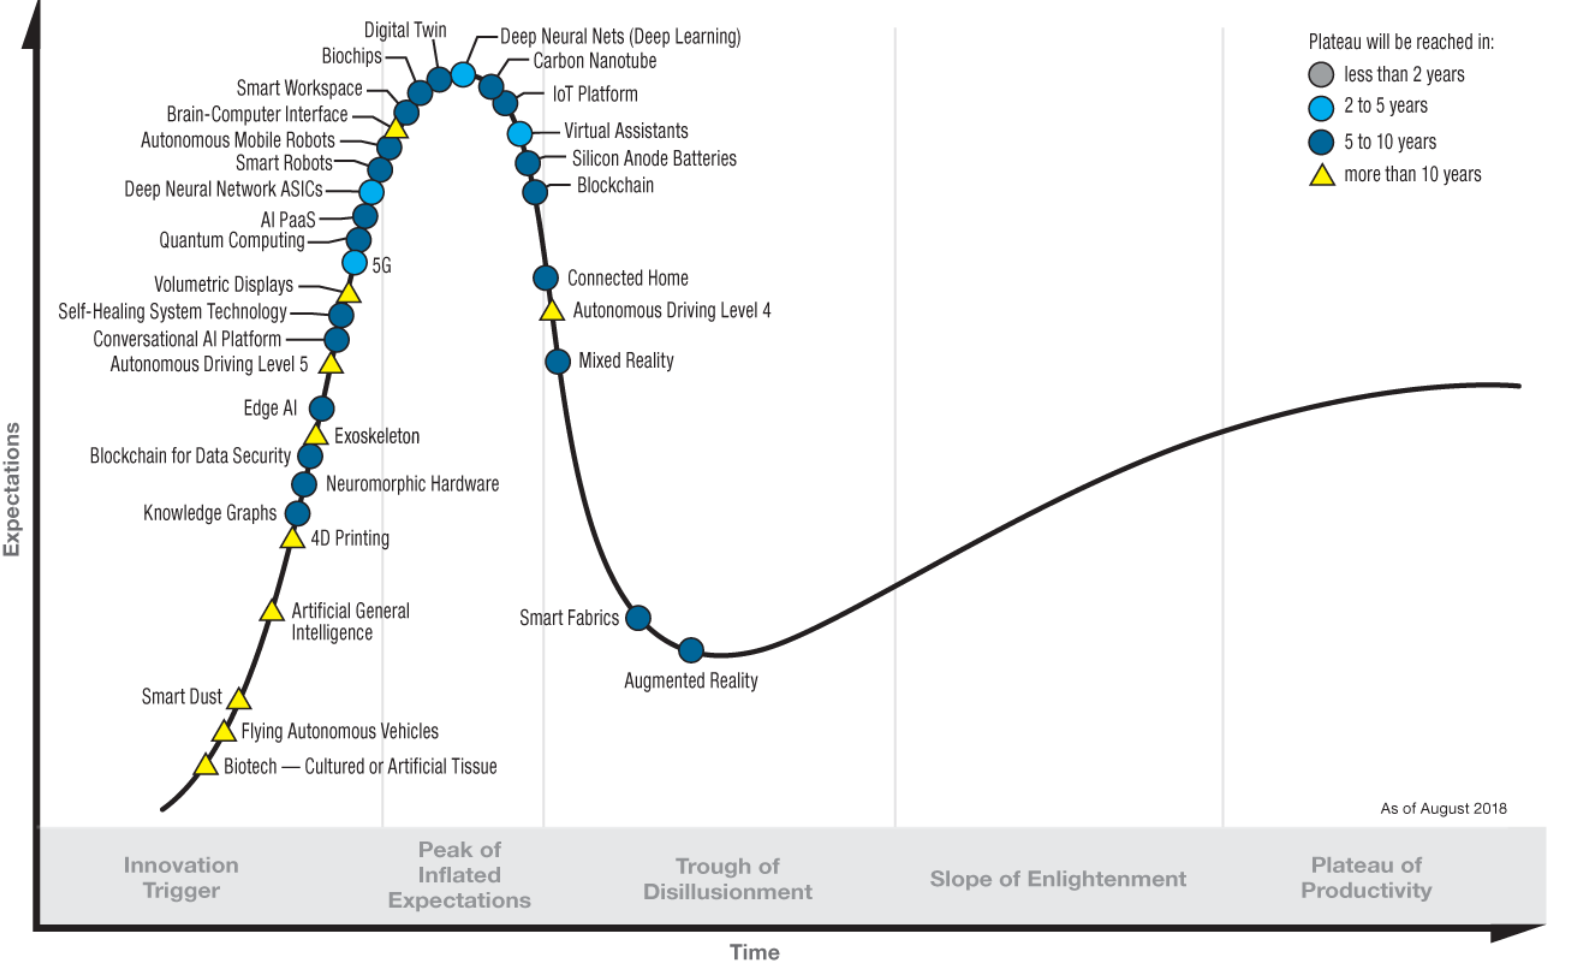
\includegraphics[scale=0.3]{background/HypeCurve.png}
      \caption{The Gartner Hype Cycle for Current Emerging Technologies
      \citep{HypeCurve}}
      \label{HypeCurveImg}
\end{figure}
%%%%%%%%%%%%%%%%%%%%%%%%%%%%%%%%%%%%%%%%


 
The hype curve has five main stages that can be briefly described as:
 
\begin{enumerate}
\item \textbf{Technology Trigger Stage:} The technology trigger stage is when the technology is first being introduced and researched.

\item \textbf{Peak of Inflated Expectation:} The peak of inflated expectation is the point at which the technology is being
adopted by mass consumers. At this stage, there are high hopes and expectations for future implementations.

\item \textbf{Trough of Disillusionment:} At the trough of disillusionment stage, the technology in question is mostly abandoned by mainstream users and they are disillusioned as to its future prospects.

\item \textbf{Slope of Enlightenment:} During the slope of enlightenment the ‘new’ technology is having a slow resurgence and is beginning to show long term potential.

\item \textbf{Plateau of Productivity:} The plateau of productivity is the final stage, where the technology does not seem to have any new improvements in prospect, and it appears that future work would be unlikely to contribute significant changes.
\end{enumerate}

It could be said that Quantum Computing is entering into Stage Two of the hype cycle, and that this movement -- from a research-centred stage towards more widespread usage -- can be attributed to the wider availability of quantum cloud computers and to the increasing number of publications that include practical implementations. However, there are still few publications that provide a detailed implementation
%centralised means of implementing a quantum machine learning circuit from the
of a quantum machine learning solution\footnote{Commonly referred to as a QEML circuit.} from the
data encoding stage to the algorithm design stage, through to the analysis of the execution results. 


\section{Quantum Enhanced Machine Learning}
A QML or QEML circuit consists of three components: the data encoding, the quantum algorithm and the measurement. 



%%%%%%%%%%%%%%%%%%%%%%%%%%%%%%%%%%%%%%%%
\begin{figure}[H]
      \centering
      %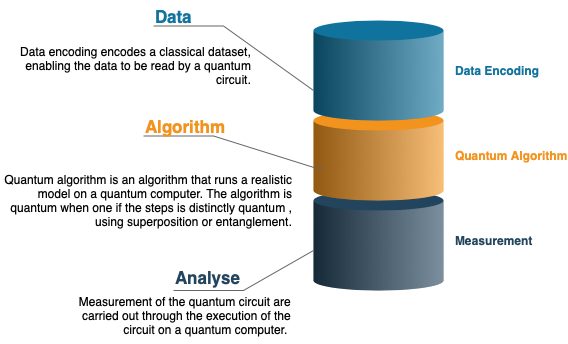
\includegraphics[scale=0.6]{background/GenLayout.png}
      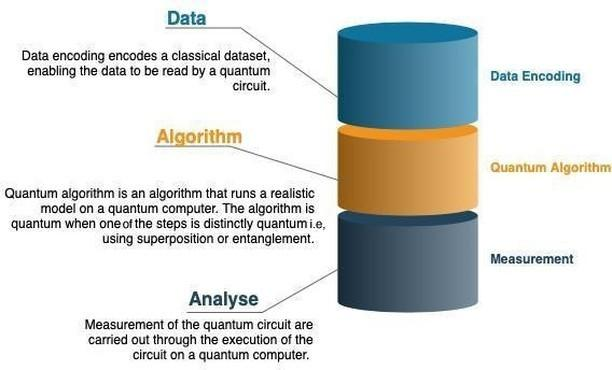
\includegraphics[scale=0.6]{background/GenLayoutFix.jpeg}
      %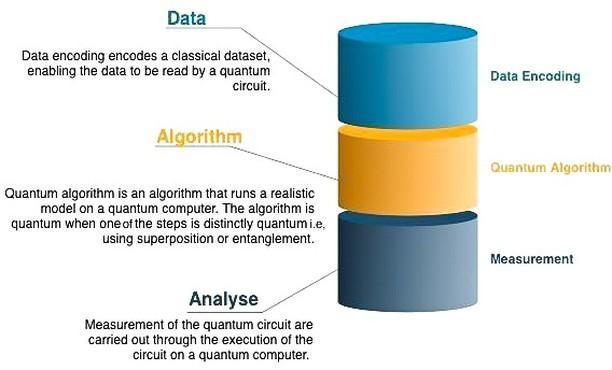
\includegraphics[scale=0.6]{background/GenLayoutFixBri.jpeg}
      \caption{General Layout of a Quantum Circuit}
      \label{GenLay}
\end{figure}
%%%%%%%%%%%%%%%%%%%%%%%%%%%%%%%%%%%%%%%%

In the data encoding component, a classical dataset is encoded into quantum data; this allows the quantum algorithm %(encoded in the quantum circuit) 
to read the encoded data as an input. After the execution of the QML circuit on a quantum machine, the output is then measured and analysed.

In this work an analysis of modular implementations of QEML and QML circuits is undertaken, based on the structure illustrated in Figure \ref{GenLay}. However, before we can discuss the implementations of the different components, we need to familiarise ourselves with the necessary quantum background. In the next section recent publications are reviewed and considered.

\subsection{Related Works}

%There exists an %wide
%array of research papers on the various quantum machine learning algorithms and circuitry topics, most of which are very theoretical or contain theoretically heavy implementations. 
An influential paper in the field of QML is 
\emph{An introduction to quantum machine learning}
%by M.~Schuld, F.~Petruccione and I.~Sinayskiy
\citep{research1}. This provides a systematic overview of the emerging field of quantum machine learning by presenting approaches and technical details in an accessible manner. 
While it details Quantum k-Nearest Neighbour (QkNN) and Quantum Support Vector Mechanism (QSVM) algorithms and the concepts behind their design, and while it outlines how to potentially implement them, it does not provide circuit details, circuit implementations using datasets, nor does it analyse QkNN or QSVM circuit outputs. It is rather an introduction that aims to provide an overview of existing ideas and approaches to quantum machine learning. 

Another very influential paper is \emph{A Computer Science-Oriented Approach to Introduce Quantum Computing to a New Audience}
%by O.~Salehi, Z.~Seskir, I.~Tepe
\citep{research2}. This paper is \emph{``an alternative educational approach for introducing quantum computing to a wider audience. It considers quantum computing as a generalised probability theory rather than a field emanating from physics, and it utilises quantum programming as an educational tool to reinforce the learning process.''}
Similarly to \citeauthor{research1}'s paper referred to above,
%Similar to the aforementioned \emph{Introduction to Quantum} research paper,
this paper does not provide code implementations nor does it consider the outputs of quantum algorithms for given datasets. Furthermore, the paper does not explore QkNN, QSVM or any other quantum algorithms. It aims, rather, to \emph{``inform academics and organisations interested in introducing quantum computing to a diverse group of participants from an educational approach''} \citep{research2}.

Chapter \ref{BackgroundLit} has a similar aim to these research papers, which is to provide an accessible introduction into the background needed for quantum computing for a software engineering audience through a non physics based approach. It is more similar to the approach used in
%\emph{An Introduction to Quantum Machine Learning}
\citeauthor{research1}'s
paper, as this chapter examines quantum machine learning algorithms like QSVM and QkNN along with Grover’s Search algorithm. %This work expands further on these research papers by exploring the other two components,
Data encoding and output measurements are also explored in this chapter, as detailed Figure \ref{GenLay}.

Quantum machine learning algorithms can not read classical datasets -- they require quantum encoded data. The above publications do not explore quantum data encoding. Papers by \citeauthor{softIntro}
%and \emph{When Machine Learning Meets Quantum Computers: A Case Study} by W.~Jiang, J.~Xiong and Y.~Shi \citep{softIntro}
and by \citeauthor{Khan2019} %\citep{Khan2019}
% and \emph{Quantum K means Algorithm} by S.U.KHAN \citep{Khan2019}
explore quantum data encoding techniques from a theoretical and practical standpoint.

% paragraph on both individually, one on each. 

\emph{When Machine Learning Meets Quantum Computers: A Case Study} \citep{softIntro}, demonstrates a framework for implementing neural networks on quantum circuits by providing a data pre-processing implementation using Tensorflow \citep{tensorflow}, along with neural computation acceleration and data post-processing code for a quantum cloud based computer. 
Practical code implementations for data encoding are provided, and the MNIST dataset \citep{deng2012mnist} is used to evaluate the data encoding methods. This paper details data encoding through the use of Tensorflow and the \texttt{transforms} function in the PyTorch \citep{paszke2017automatic} Torchvisions \citep{torchvision}  library to modify data features. The paper provides a framework for a quantum neural network circuit, providing code implementations corresponding to the data encoding and the measurement modules in Figure \ref{GenLay}, where a two layer quantum neural network implementation provides the the quantum algorithm component. Nevertheless, it is just a framework -- it does not execute any of the components on a quantum computer, nor does it evaluate their resulting output.

In their thesis entitled \emph{Quantum k Means Algorithm} \citeauthor{Khan2019} \emph{``explores the quantum implementation of K-means clustering algorithm and propose three optimization strategies to achieve shorter-depth circuits for quantum K-means on NISQ \citep{NISQ} \footnote{Noisy intermediate-scale quantum (NISQ) algorithms. We are far from a universal fault-tolerant quantum computer, it will potentially take decades to reach that standard. NISQ computers are here right now, though they have hundreds of noisy bits, they can leverage limited quantum resources in order to preform classically challenging tasks. }  computers.''} \citep{Khan2019}.
Amplitude data encoding is used in the quantum implementations of the k Means algorithm to perform clustering using shallow depth quantum circuits. Where \citeauthor{softIntro} details the use of the MNIST dataset for quantum encoding, this paper employs both the MNIST and the Iris datasets \citep{IrisDataset}, and evaluates the circuit algorithms on a Qiskit \citep{Qiskit-koch2019introduction} quantum cloud based computer.
%More than one implementation for a quantum algorithm is explored in the paper, detailing both
Single cluster and multi cluster quantum k Means implementations are explored in the paper. %through the use of circuit illustrations.
However, code for these implementations is not provided.

This work will provide the circuit diagrams and the code necessary to implement two variations of data encoding, along with multiple quantum algorithms and modular implementation of these algorithms.




%Both papers provide an implementation for data encoding, with S.U.~KHAN et al (2020) making use for amplitude encoding when detailing quantum implementations for the k Means algorithm to perform clustering using shallow depth quantum circuits. While W.~Jiang, J.~Xiong and Y.~Shi et al (2020), demonstrate a framework for implementing neural networks onto quantum circuits, by a providing data pre-processing implementation using tensor flow, along with neural computation acceleration and data post-processing code \citep{softIntro}.

%Both encoding methods are applied to the MINST dataset however, only S.U.KHAN et al (2020) applies these datasets to a quantum algorithm, k Means quantum algorithm, which is then analysed using a quantum computer.  S.U.KHAN et al (2020) also implements both single cluster and multi cluster quantum k Means through the use of circuit illustrations however, it does not provide code for these implementations, only proposed circuit diagrams. While W.Jiang, J.Xiong and Y.Shi et al (2020) does provide practical code implementations for data encoding, it does not detail circuit diagrams and it does not perform the measurement stage in Figure \ref{GenLay}. This work will provide the circuit diagrams and the code necessary to implement two variations of data encoding and the quantum algorithms for these circuits. 

There are publications that provide all three components shown in Figure \ref{GenLay}, while also making use of circuit diagrams or code snippets, these are \emph{Building a Quantum kNN Classifier with Qiskit: theoretical gains put to practice} by D.J.~Kok \citep{INGKOK} and \emph{ QEML:(Quantum Enhanced Machine Learning) Using Quantum Computation to implement a K-nearest Neighbours Algorithm in a Quantum Feature Space on Superconducting Processors} by \cite{sharmaQeml}.

\cite{sharmaQeml} implements the quantum-enhanced version of the k-Nearest Neighbours algorithm, making use of the same QkNN version implemented in this work, the Hamming distance. This paper also explores multiple datasets namely, the Iris and the Wisconsin Cancer datasets. However, it only evaluates the QkNN circuit using 10 data points from these datasets, as the method for data encoding, maps each datapoint to a quantum gate. This encoding method restricts the number of data points that can be used, based on the current number of qubits available on a quantum computer. \footnote{The current largest quantum machine that is open to non institutional use is limited to 15 qubits.}
\citeauthor{sharmaQeml} also evaluates the QkNN circuit on a quantum simulator, instead of using a real quantum device.


\citeauthor{INGKOK} implements a version of QkNN  capable of performing kNN classification using the Dot Product method. Similar to \citep{sharmaQeml}, this paper makes use of the Iris dataset, but also the Hofmann (German Credit dataset) and the HEP datasets. It also incorporates more data points into the output evaluation as it makes use of the analog encoding technique, which normalises the data points and allows for data to be encoding into a smaller number of qubits. However, both \citeauthor{sharmaQeml}'s paper and  \citeauthor{INGKOK} paper evaluates the QkNN circuit using only a simulated quantum device, this paper executes the quantum circuit on a quantum cloud based computer.


While both publications detail QML implementations for a singular quantum algorithm and data encoding technique, \citeauthor{INGKOK} only implements QkNN using the Qsiksit built-in function.  
This work incorporates the Qiskit built in function but it also provides the Hamming distance circuit implementation found in \citeauthor{sharmaQeml}. These QkNN implementations are illustrated in Section \ref{ImpleQkNN} as part of the modular design for the circuit, along with two implementations for data encoding that are similarly evaluated using multiple datasets. 





\section{Motivation}

When one first begins to study quantum computing with the aim of writing quantum programs, one will learn about: the different quantum machine learning and quantum based algorithms, how to run a circuit on a quantum machine and possibly data encoding techniques from one of the aforementioned publications. The ability to see all the necessary stages and different components that could be implemented is not centralised.

Taking the first stage -- data encoding -- most publications and bodies of work, including those mentioned, do not provide both the code needed for implementing them and their circuit illustrations. Finding both of these for more than one data encoding technique and for more than a single quantum machine algorithm, was not found during the research stage of this dissertation. Taking the quantum library Qiskit as an example, particularly their documentation and instructional videos, it can be noted that the documentation provides function calls for data encoding, while the videos focus on different quantum algorithm implementations with code that calls their built in “black box” functions.
%Qiskit's resources, similar to other quantum circuit publications, 
It does not detail, within the same resource location, how to incorporate all the stages shown in Figure \ref{GenLay} into a full QML circuit, or how each of these components operate. 

The intention of this dissertation is to deliver the various stages in a quantum system by implementing the various theoretical research methods that can be found across different publications, and by presenting them in a layout that can be configured with these components in a modular manner. Thus providing software engineers, who may be new quantum users, with the ability to combine different data encoding techniques with different quantum algorithms as they learn. It also provides a modular foundation for more quantum algorithms, such as k Means, to be added to the modular circuit and tested with the existing modular data encoding components or, for additional data encoding techniques such as digital encoding to be incorporated in the same manner. 


\section{Method}

The publications explored provide partial or complete stages of a QML circuit, only focused on the implementation of one component of each. As illustrated in Figure \ref{ImpleLayout}, this work will explore each step of a quantum circuit and provide options for each stage and the modular code needed for their implementation. 


%%%%%%%%%%%%%%%%%%%%%%%%%%%%%%%%%%%%%%%%
\begin{figure}[h!]
      \centering
      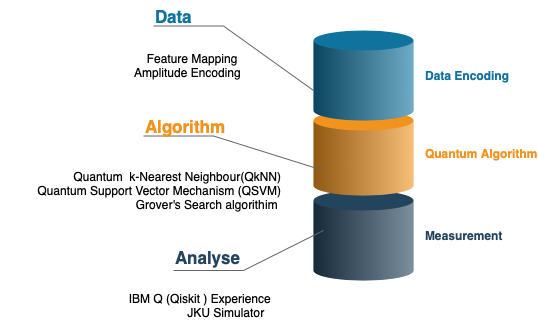
\includegraphics[scale=0.6]{background/MyLayoutImple.png}
      \caption{Layout of a Quantum Circuit Components Implemented}
      \label{ImpleLayout}
\end{figure}
%%%%%%%%%%%%%%%%%%%%%%%%%%%%%%%%%%%%%%%%


To achieve this, the following contributions are made in this dissertation:

\begin{itemize}
\item

The first and the most important aim is to provide a circuit with all three stages found in Figure \ref{ImpleLayout} with modular components in an accessible form. This enables future development on this work to be easy and approachable, particularly for quantum enthusiasts and those more literate in software development than in quantum physics. To do so, the necessary python code is presented in a technical manner where detailed knowledge of quantum physics would not be necessary. However, the basic quantum theoretical knowledge will be explained in a concise and austere style.

\end{itemize}

\begin{itemize}
\item
For the algorithm stage of the circuit, a full quantum machine learning  %variating
implementation of k-Nearest Neighbour is detailed based on the descriptions detailed in the work \emph{ Algorithm for k-Nearest Neighbours Classification based on the Metric of Hamming Distance} (12) \citep{sharmaQeml}. %, while the other implementation incorporates the Qiskit built in function used in \citep{sharmaQeml}. 
Two variations of Grover’s Search algorithm and QSVM are also explored, these are delivered through illustrative and succinct implementations.

\end{itemize}


\begin{itemize}
\item

As previously stated, in order to run classical data on a quantum circuit, quantum readable data is required. Existing data encoding methods, both theoretical and implemented, are dispersed across various research publications. This work presents different methods for data encoding both the circuit design and the code in a centralised location.


\end{itemize}


\begin{itemize}
\item

Finally, bench-marking is performed on the aforementioned quantum machine learning algorithms and their classical counterparts. Similar to the publications we explored, the circuit is analysed using multiple datasets with various data points, executed on a quantum computer. In addition to the quantum computer execution, this work details an external classical quantum based simulator, the JKU simulator, its advantages, current state and the necessary implementation. These measurement techniques allow for a critical review of the circuit results, for the different circuit components.

\end{itemize}